\begin{figure}[H]
  \centering
  \captionsetup[subfigure]{labelformat=empty}
  \setkeys{Gin}{width=2.5in,height=2.5cm,keepaspectratio}%
  \subfloat[Obj. 1a]{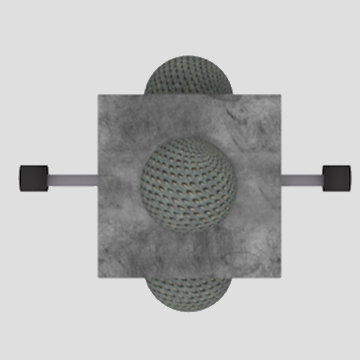
\includegraphics{Bilder/Objekt1A.png}}
  \hspace{0.5cm}
  \subfloat[Obj. 1b]{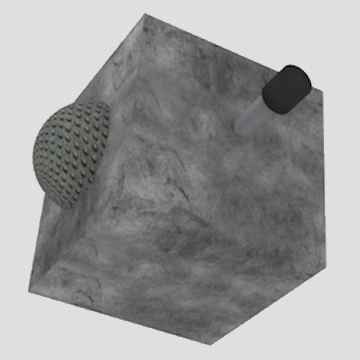
\includegraphics{Bilder/Objekt1B.png}} 
  \hspace{0.5cm}
  \subfloat[Obj. 2a]{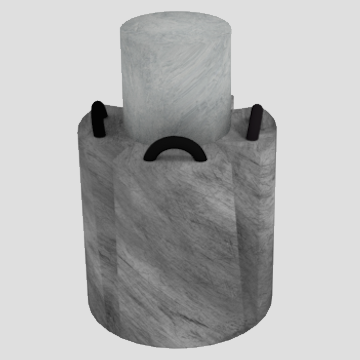
\includegraphics{Bilder/Objekt2A.png}}
  \hspace{0.5cm}
  \subfloat[Obj. 2b]{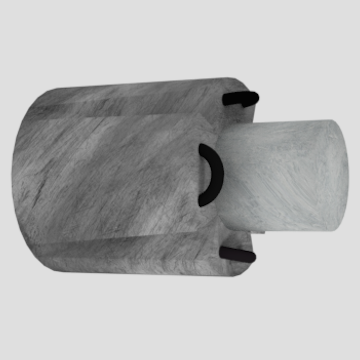
\includegraphics{Bilder/Objekt2B.png}} \\
  \subfloat[Obj. 3a]{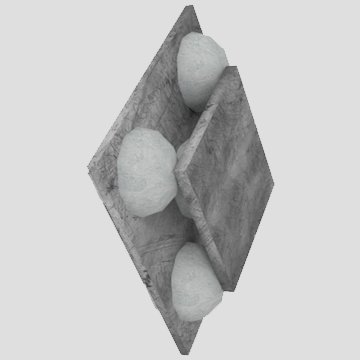
\includegraphics{Bilder/Objekt3A.png}}
  \hspace{0.5cm}
  \subfloat[Obj. 3b]{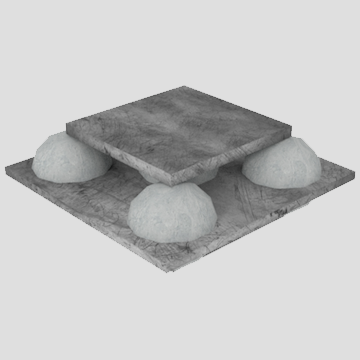
\includegraphics{Bilder/Objekt3B.png}}
  \hspace{0.5cm}
  \subfloat[Obj. 4a]{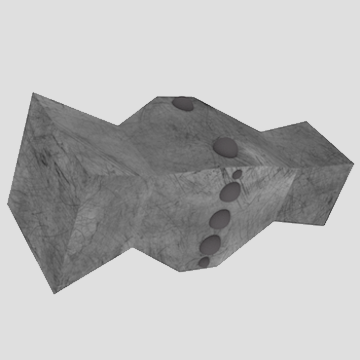
\includegraphics{Bilder/Objekt4A.png}}
  \hspace{0.5cm}
  \subfloat[Obj. 4b]{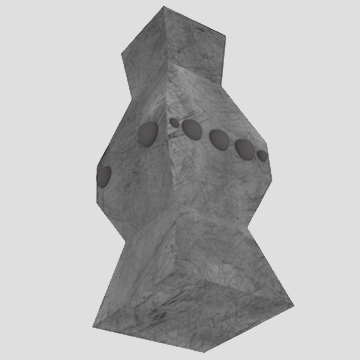
\includegraphics{Bilder/Objekt4B.png}}\\
    \subfloat[Obj. 5a]{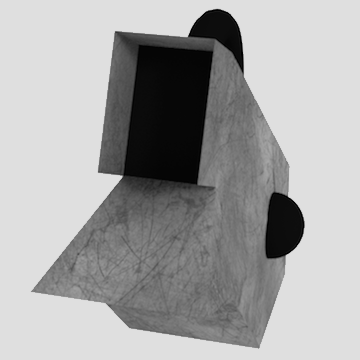
\includegraphics{Bilder/Objekt5A.png}}
  \hspace{0.5cm}
  \subfloat[Obj. 5b]{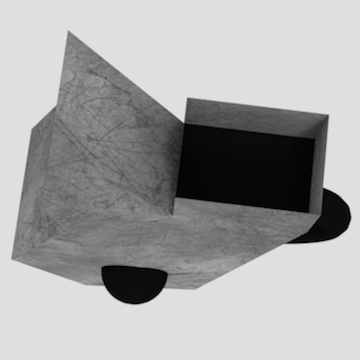
\includegraphics{Bilder/Objekt5B.png}}
  \hspace{0.5cm}
  \subfloat[Obj. 6a]{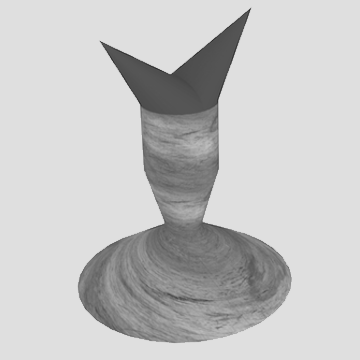
\includegraphics{Bilder/Objekt6A.png}}
  \hspace{0.5cm}
  \subfloat[Obj. 6b]{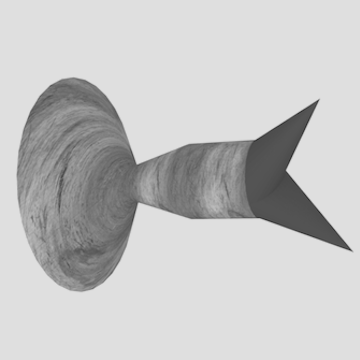
\includegraphics{Bilder/Objekt6B.png}}\\
   \subfloat[Obj. 7a]{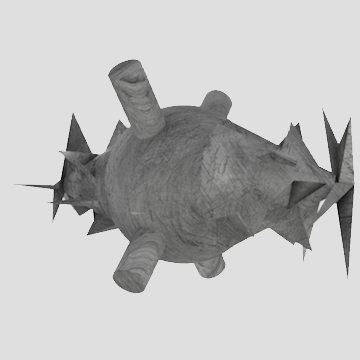
\includegraphics{Bilder/Objekt7A.png}}
  \hspace{0.5cm}
  \subfloat[Obj. 7b]{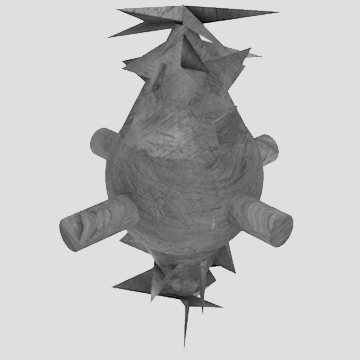
\includegraphics{Bilder/Objekt7B.png}}
  \hspace{0.5cm}
  \subfloat[Obj. 8a]{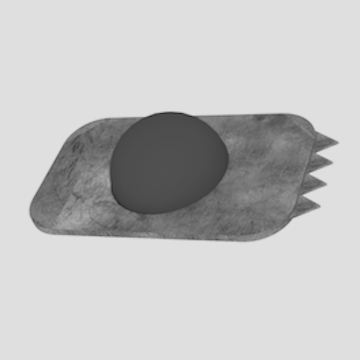
\includegraphics{Bilder/Objekt8A.png}}
  \hspace{0.5cm}
  \subfloat[Obj. 8b]{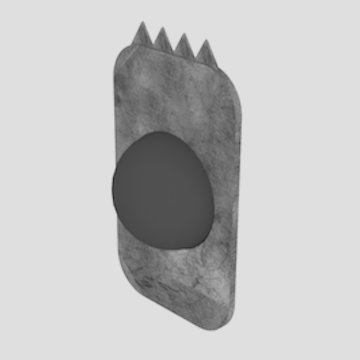
\includegraphics{Bilder/Objekt8B.png}}\\
    \subfloat[Obj. 9a]{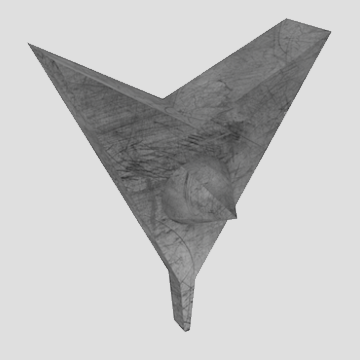
\includegraphics{Bilder/Objekt9A.png}}
  \hspace{0.5cm}
  \subfloat[Obj. 9b]{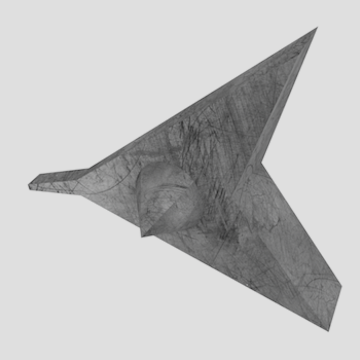
\includegraphics{Bilder/Objekt9B.png}}
  \hspace{0.5cm}
  \subfloat[Obj. 10a]{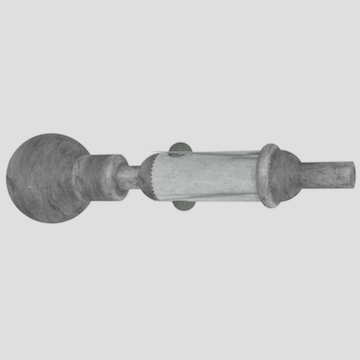
\includegraphics{Bilder/Objekt10A.png}}
  \hspace{0.5cm}
  \subfloat[Obj. 10b]{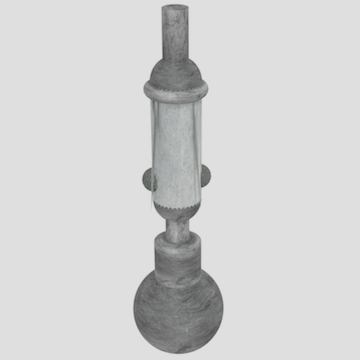
\includegraphics{Bilder/Objekt10B.png}}
  \caption{Note. a = originale Ausrichtung, b = rotiert}
\end{figure}

\begin{figure}[H]
  \ContinuedFloat\centering
  \captionsetup[subfigure]{labelformat=empty}
  \setkeys{Gin}{width=2.5in,height=2.5cm,keepaspectratio}%
   \subfloat[Obj. 11a]{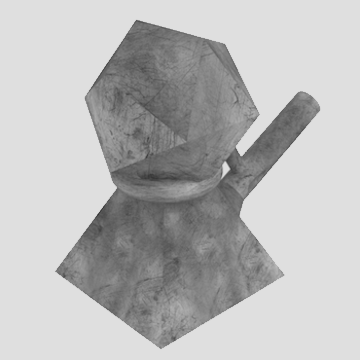
\includegraphics{Bilder/Objekt11A.png}}
  \hspace{0.5cm}
  \subfloat[Obj. 11b]{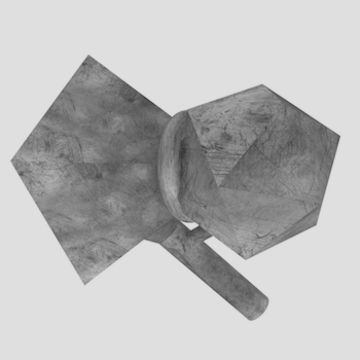
\includegraphics{Bilder/Objekt11B.png}}
  \hspace{0.5cm}
  \subfloat[Obj. 12a]{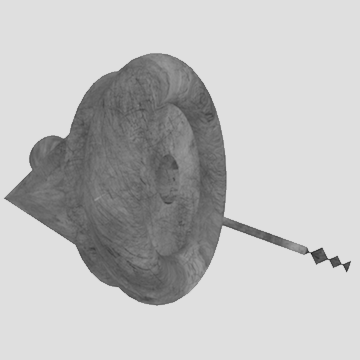
\includegraphics{Bilder/Objekt12A.png}}
  \hspace{0.5cm}
  \subfloat[Obj. 12b]{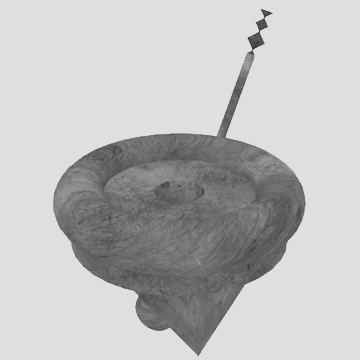
\includegraphics{Bilder/Objekt12B.png}}\\
   \subfloat[Obj. 13a]{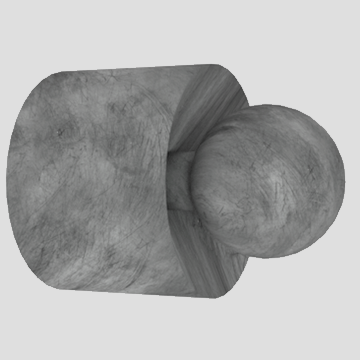
\includegraphics{Bilder/Objekt13A.png}}
  \hspace{0.5cm}
  \subfloat[Obj. 13b]{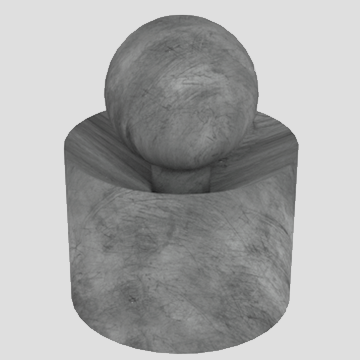
\includegraphics{Bilder/Objekt13B.png}}
  \hspace{0.5cm}
  \subfloat[Obj. 14a]{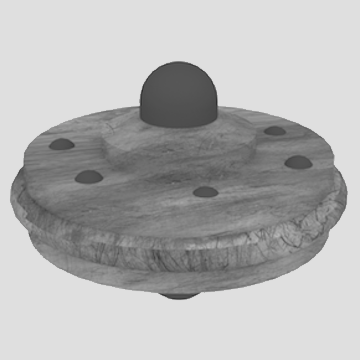
\includegraphics{Bilder/Objekt14A.png}}
  \hspace{0.5cm}
  \subfloat[Obj. 14b]{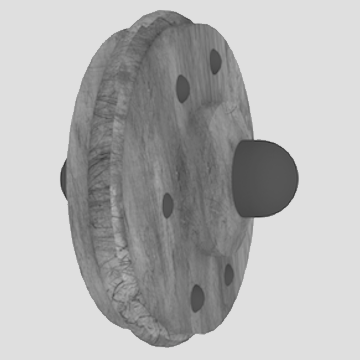
\includegraphics{Bilder/Objekt14B.png}}\\
  \end{figure}
  
  \begin{figure}[H]
  \ContinuedFloat\centering
  \captionsetup[subfigure]{labelformat=empty}
  \setkeys{Gin}{width=2.5in,height=2.5cm,keepaspectratio}%
   \subfloat[Obj. 15a]{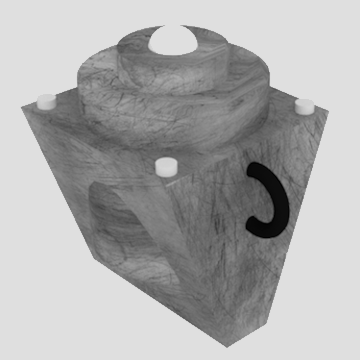
\includegraphics{Bilder/Objekt15A.png}}
  \hspace{0.5cm}
  \subfloat[Obj. 15b]{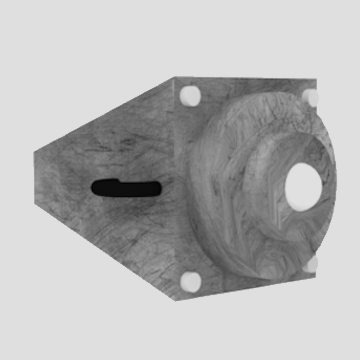
\includegraphics{Bilder/Objekt15B.png}}
  \hspace{0.5cm}
  \subfloat[Obj. 16a]{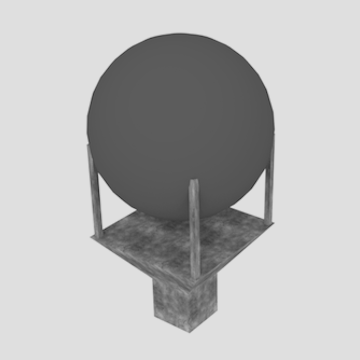
\includegraphics{Bilder/Objekt16A.png}}
  \hspace{0.5cm}
  \subfloat[Obj. 16b]{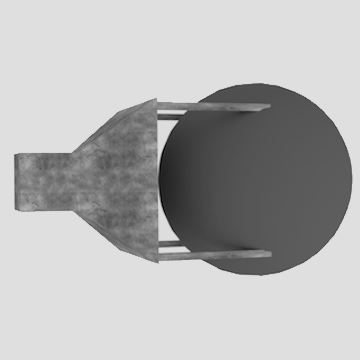
\includegraphics{Bilder/Objekt16B.png}}\\
   \subfloat[Obj. 17a]{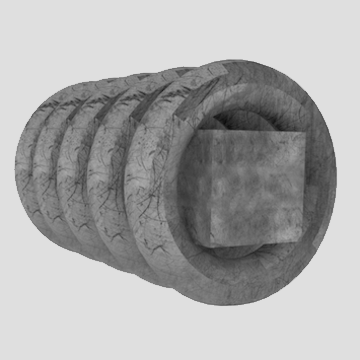
\includegraphics{Bilder/Objekt17A.png}}
  \hspace{0.5cm}
  \subfloat[Obj. 17b]{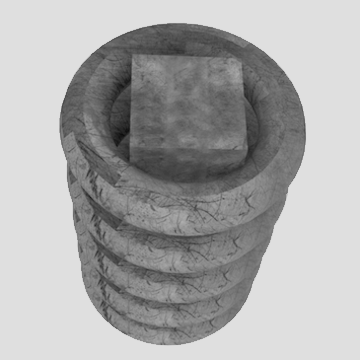
\includegraphics{Bilder/Objekt17B.png}}
  \hspace{0.5cm}
  \subfloat[Obj. 18a]{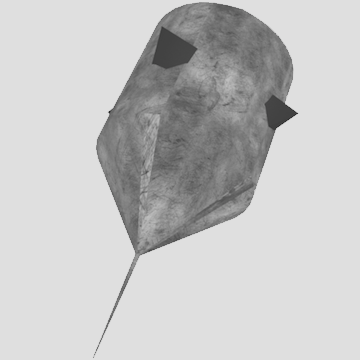
\includegraphics{Bilder/Objekt18A.png}}
  \hspace{0.5cm}
  \subfloat[Obj. 18b]{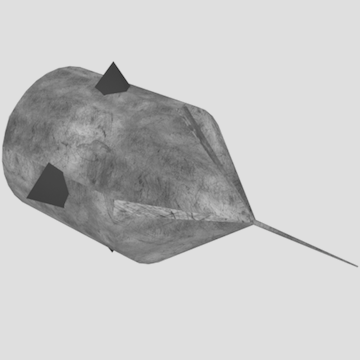
\includegraphics{Bilder/Objekt18B.png}}\\
  \caption{Note. a = originale Ausrichtung, b = rotiert}
\end{figure}